\section{MVA analysis}
\label{sec:mva}

In this section, we investigate the sensitivity of probing signal using one of the Multi-Variate Analysis (MVA) methods, the Gradient Boosted Decision Trees (BDT) method~\cite{BDT,BDT2}, with the {\tt TMVA} software package. The BDT output score is in the range between -1 and 1. The most signal-like events have scores near 1 while the most background-like events have scores near -1.

The signal topology and kinematics are different across all the channels. To maximize the overall sensitivity, separated BDTG trainings are applied to each the signal region. A number of variables as the BDT inputs are used to train and test events in each signal region for maximal signal acceptance and background rejection. They are listed in Tab.~\ref{tab:mva_var}. 

\begin{table}[htp]
\caption{The BDT input variables (checkmarked) used in each FR. }
\centering
\begin{tabular}{|c|cc|cc|c|} \hline
  & \multicolumn{2}{c|}{$\tlhad+$ jets} & \multicolumn{2}{c|}{$\thadhad+$ jets} & $\thadhad+l$\\ \cline{2-6}
 & 3 jets & >=4 jets & 3 jets & >=4 jets & >=1 jet\\ \hline
$m_{\tau\tau}^{\text{fit}}$                      	& \checkmark  & \checkmark  & \checkmark  & \checkmark & \\
$E^{\text{T}}_{\text{miss}}$                                	& \checkmark  & \checkmark  & \checkmark  & \checkmark &\\
$p_{\text{T},\text{lead}-\tau}$                               & \checkmark  & \checkmark  &  \checkmark & \checkmark & \checkmark\\
$p_{\text{T},\text{sublead}-\tau}$                               & \checkmark  & \checkmark  & \checkmark & \checkmark & \checkmark\\
$\Delta\phi(\tau\tau,P^{\text{T}}_{\text{miss}})$                             	& \checkmark & \checkmark & \checkmark  & \checkmark &\\
$m_{\tau\tau,\text{vis}}$                             	& \checkmark  & \checkmark  & \checkmark  & \checkmark & \checkmark\\
$\met$ centrality                             	& \checkmark  & \checkmark  & \checkmark  & \checkmark &\\
$\Delta R(\tau,\tau)$                   		        & \checkmark  & \checkmark  & \checkmark  & \checkmark & \checkmark\\
$\Delta R(\tau,\text{light-jet},\text{min})$      			        & \checkmark  & \checkmark  & \checkmark & \checkmark & \checkmark\\
$m_{t,\text{SM}}$                   &         & \checkmark  &          & \checkmark &\\
$m_{t,\text{FCNC}}$                   & \checkmark & \checkmark  & \checkmark & \checkmark &\\
$x_1^{\text{fit}}$				& \checkmark  &	\checkmark  & \checkmark  & \checkmark &\\
$x_2^{\text{fit}}$				& \checkmark  & \checkmark  & \checkmark  & \checkmark &\\
$\Delta R(l,\tau) $  &           &         &       &     & \checkmark\\
$\eta_{\tau,\text{max}} $  &           &         &       &     & \checkmark\\
$\mtw $  &           &         &       &     & \checkmark\\
$\Delta R(l+b\text{-jet},\tau\tau) $  &           &         &       &     & \checkmark\\ 
$m_{t,\text{FCNC,vis}}$                   &   &    &   &   & \checkmark\\
$m_{t,\text{SM,vis}}$                   &           &         &       &     & \checkmark\\
$P_{\text{t,vis}}^{\tau\tau}$                      &           &         &       &     & \checkmark\\\hline
\end{tabular}
\label{tab:mva_var}
\end{table}

The signal and background samples are randomly divided into two equal parts (denoted as even and odd parity events). The BDT is trained with one part, and tested on the other part. It is always ensured that the BDT derived from the training events is not applied to the same events, but only to the independent test ones. The sum of all background processes, corrected normalized, are used in the training and testing. The Gradient BDT parameters used are listed in Tab. \ref{tab:bdt_pars}. With the \texttt{IgnoreNegWeightsInTraining} option, only MC events with positive MC weights are used in the traning. The comparison of BDT performances in test-odd and test-even samples is given in Fig. \ref{fig:overtrain}. The BDT parameters \texttt{NTrees} and \texttt{nCuts} are tuned such that the test-odd and test-even agrees, and the signal sensitivity is optimised.

%\begin{table}
%\caption{The Gradient BDT hyper parameters used in each FR. }
%\centering
%\begin{tabular}{|c|c|c|c|} \hline
%  & \texttt{NTrees} & \texttt{Shrinkage} & \texttt{BaggedSampleFraction} \\ \hline
%   $\tlhad$ 3-jet & 500 & \multirow{4}{*}{0.1} & \multirow{4}{*}{0.6} \\ \cline{1-2}
%   $\tlhad$ 4-jet & 700 &  &  \\ \cline{1-2}
% $\thadhad$ 3-jet & 600 &  &  \\ \cline{1-2}
% $\thadhad$ 4-jet & 800 &  &  \\ \hline\hline
%  & \texttt{nCuts} & \texttt{MaxDepth} & \texttt{NegWeightTreatment} \\ \hline
%   $\tlhad$ 3-jet & 20 & \multirow{4}{*}{2} & \multirow{4}{*}{\texttt{IgnoreNegWeightsInTraining}} \\ \cline{1-2}
%   $\tlhad$ 4-jet & 20 &  & \\ \cline{1-2}
% $\thadhad$ 3-jet & 15 &  & \\ \cline{1-2}
% $\thadhad$ 4-jet & 15 &  & \\ \hline
%\end{tabular}
%\label{tab:bdt_pars}
%\end{table}

%\texttt{NTrees=1000::BoostType=Grad:Shrinkage=0.1:UseBaggedBoost:BaggedSampleFraction=0.5\\:nCuts=20:MaxDepth=2}.

The seperation\footnote{
The separation is defined by, as in \cite{BDT2},
\begin{equation}
\langle S^2 \rangle = \frac{1}{2} \int \frac{\left[p_S(y)-p_B(y)\right]^2}{p_S(y)+p_B(y)} dy,
\end{equation}
where $p_S(y)$ and $p_B(y)$ are the signal and background PDFs of the classifier $y$. The separation is 0 (1) for identical (non-overlapping) signal and background shapes.
} and importance\footnote{
The importance is evaluated as the total separation gain that this variable had in the decision trees (weighted by the number of events). It is normalized to all variables together, which have an importance of 1.
}
of different variables used in the training are listed in Tab. \ref{tab:mva_sep_imp_lh_3j}-\ref{tab:mva_sep_imp_hh_4j}. The last two variables in the importance ranking are moved to check the impact on the MVA performance, and the results can be found in App. \ref{app:mva_input_var}. 

The distributions of the variables with the largest importance are shown in Fig. \ref{fig:mva_input}.
\begin{table}
\caption{The Separation and Importance of different variables used in the training for STH $\tlhad$ category.}
\centering

\begin{tabular}{|c|c|} \hline
 & Importance \\ \hline

$\drtautau      $ & $1.022\times10^{-1}$ \\
$\taupto        $ & $1.001\times10^{-1}$ \\
$\ttvismass     $ & $9.796\times10^{-2}$ \\
$\etmiss        $ & $9.766\times10^{-2}$ \\
$\drtaujmin     $ & $9.375\times10^{-2}$ \\
$\met$ centrality & $8.673\times10^{-2}$ \\
$\xlfit         $ & $7.750\times10^{-2}$ \\
$\dphitauetmiss $ & $7.690\times10^{-2}$ \\
$\tautaumass    $ & $7.321\times10^{-2}$ \\
$\tzmass        $ & $7.089\times10^{-2}$ \\
$\xzfit         $ & $6.434\times10^{-2}$ \\
$\tauptl        $ & $5.874\times10^{-2}$ \\\hline

\end{tabular}
\label{tab:mva_sep_imp_lh_3j}
\end{table}

\begin{table}
\caption{The Separation and Importance of different variables used in the training for TTH $\tlhad$ category.}
\centering
\begin{tabular}{|c|c|} \hline
 & Importance \\ \hline
$\ttvismass     $ & $9.658\times10^{-2}$ \\
$\taupto        $ & $9.449\times10^{-2}$ \\
$\drtautau      $ & $9.045\times10^{-2}$ \\
$\etmiss        $ & $8.637\times10^{-2}$ \\
$\tautaumass    $ & $8.353\times10^{-2}$ \\
$\drtaujmin     $ & $7.600\times10^{-2}$ \\
$\dphitauetmiss $ & $7.475\times10^{-2}$ \\
$\met$ centrality & $7.357\times10^{-2}$ \\
$\xlfit         $ & $6.675\times10^{-2}$ \\
$\tzmass        $ & $6.511\times10^{-2}$ \\
$\xzfit         $ & $5.272\times10^{-2}$ \\
$\tauptl        $ & $4.691\times10^{-2}$ \\
$\tlmass        $ & $4.671\times10^{-2}$ \\
$\wmass         $ & $4.606\times10^{-2}$ \\\hline

\end{tabular}
\label{tab:mva_sep_imp_lh_4j}
\end{table}

\begin{table}
\caption{The Separation and Importance of different variables used in the training for STH $\thadhad$ category.}
\centering
\begin{tabular}{|c|c|} \hline
 & Importance \\ \hline
$\tautaumass    $  & $9.937\times10^{-2}$  \\ \hline
$\ttvismass     $  & $9.904\times10^{-2}$  \\ \hline
$\tlmass        $  & $8.786\times10^{-2}$  \\ \hline
$\etmiss        $  & $8.323\times10^{-2}$  \\ \hline
$\drtaujmin     $  & $7.952\times10^{-2}$  \\ \hline
$\taupto        $  & $7.244\times10^{-2}$  \\ \hline
$\tauptl        $  & $6.678\times10^{-2}$  \\ \hline
$\tzmass        $  & $6.614\times10^{-2}$  \\ \hline
$\drtautau      $  & $6.585\times10^{-2}$  \\ \hline
$\xzfit         $  & $6.394\times10^{-2}$  \\ \hline
$\met$ centrality  & $5.735\times10^{-2}$  \\ \hline
$\dphitauetmiss $  & $5.557\times10^{-2}$  \\ \hline
$\xlfit         $  & $5.152\times10^{-2}$  \\ \hline
$\wmass         $  & $5.138\times10^{-2}$  \\ \hline


\end{tabular}
\label{tab:mva_sep_imp_hh_3j}
\end{table}

\begin{table}
\caption{The Separation and Importance of different variables used in the training for TTH $\thadhad$ category.}
\centering
\begin{tabular}{|c|c|} \hline
 & Importance \\ \hline

$\tautaumass     $  & $1.066\times10^{-1}$  \\ \hline
$\ttvismass      $  & $1.008\times10^{-1}$  \\ \hline
$\drtautau       $  & $8.598\times10^{-2}$  \\ \hline
$\tlmass         $  & $8.339\times10^{-2}$  \\ \hline
$\xzfit          $  & $7.583\times10^{-2}$  \\ \hline
$\taupto         $  & $7.551\times10^{-2}$  \\ \hline
$\tzmass         $  & $7.434\times10^{-2}$  \\ \hline
$\tauptl         $  & $7.252\times10^{-2}$  \\ \hline
$\drtaujmin      $  & $6.636\times10^{-2}$  \\ \hline
$\dphitauetmiss  $  & $6.453\times10^{-2}$  \\ \hline
$\etmiss         $  & $5.848\times10^{-2}$  \\ \hline
$\met$ centrality   & $5.803\times10^{-2}$  \\ \hline
$\xlfit          $  & $4.552\times10^{-2}$  \\ \hline
$\wmass          $  & $3.215\times10^{-2}$  \\ \hline

\end{tabular}
\label{tab:mva_sep_imp_hh_4j}
\end{table}

\begin{table}
\caption{The Separation and Importance of different variables used in the training for $l\thadhad$ channel.}
\centering
\begin{tabular}{|c|c|} \hline
 & Importance \\ \hline
$\ttvismass   $ & $1.123\times10^{-1}$ \\
$\drtautau    $ & $8.934\times10^{-2}$ \\
$\tzvismass    $ & $8.809\times10^{-2}$ \\
$\etamax      $ & $8.034\times10^{-2}$ \\
$\drltau      $ & $8.018\times10^{-2}$ \\
$\tlvismass   $ & $7.749\times10^{-2}$ \\
$\drlbditau   $ & $7.400\times10^{-2}$ \\
$\tauptl      $ & $7.328\times10^{-2}$ \\
$\taupto      $ & $7.110\times10^{-2}$ \\
$\mtw         $ & $6.980\times10^{-2}$ \\
$\drtaujmin   $ & $6.645\times10^{-2}$ \\
$\tzvismass   $ & $6.176\times10^{-2}$ \\
$\tautauvispt $ & $5.588\times10^{-2}$ \\ \hline

\end{tabular}
\label{tab:mva_sep_imp_lh_4j}
\end{table}

\begin{figure}[htb]
\centering
\includegraphics[page=6,width=0.25\textwidth]{figures/r21/thq2tau/SSOSWithFakeMCCalibrated/reg2mtau1b2jos/tautaumass.pdf}
\put(-30, 80){\textbf{(a1)}}
\includegraphics[page=6,width=0.25\textwidth]{figures/r21/thq2tau/SSOSWithFakeMCCalibrated/reg2mtau1b2jos/ttvismass.pdf}
\put(-30, 80){\textbf{(a2)}}
\includegraphics[page=6,width=0.25\textwidth]{figures/r21/thq2tau/SSOSWithFakeMCCalibrated/reg2mtau1b2jos/t1mass.pdf}
\put(-70, 70){\textbf{(a3)}}
\\
\includegraphics[page=6,width=0.25\textwidth]{figures/r21/thq2tau/SSOSWithFakeMCCalibrated/reg2mtau1b3jos/tautaumass.pdf}
\put(-30, 80){\textbf{(b1)}}
\includegraphics[page=6,width=0.25\textwidth]{figures/r21/thq2tau/SSOSWithFakeMCCalibrated/reg2mtau1b3jos/ttvismass.pdf}
\put(-30, 80){\textbf{(b2)}}
\includegraphics[page=6,width=0.25\textwidth]{figures/r21/thq2tau/SSOSWithFakeMCCalibrated/reg2mtau1b3jos/drtautau.pdf}
\put(-70, 70){\textbf{(b3)}}
\\
\includegraphics[page=6,width=0.25\textwidth]{figures/r21/thq1lntau/Wfake/doublecount/plots_NOMINAL/reg1l1tau1b2j_os/drtautau.pdf}
\put(-30, 80){\textbf{(c1)}}
\includegraphics[page=6,width=0.25\textwidth]{figures/r21/thq1lntau/Wfake/doublecount/plots_NOMINAL/reg1l1tau1b2j_os/taupt_0.pdf}
\put(-30, 80){\textbf{(c2)}}
\includegraphics[page=6,width=0.25\textwidth]{figures/r21/thq1lntau/Wfake/doublecount/plots_NOMINAL/reg1l1tau1b2j_os/tautauvismass.pdf}
\put(-70, 70){\textbf{(c3)}}
\\
\includegraphics[page=6,width=0.25\textwidth]{figures/r21/thq1lntau/Wfake/doublecount/plots_NOMINAL/reg1l1tau1b3j_os/tautauvismass.pdf}
\put(-30, 80){\textbf{(d1)}}
\includegraphics[page=6,width=0.25\textwidth]{figures/r21/thq1lntau/Wfake/doublecount/plots_NOMINAL/reg1l1tau1b3j_os/taupt_0.pdf}
\put(-30, 80){\textbf{(d2)}}
\includegraphics[page=6,width=0.25\textwidth]{figures/r21/thq1lntau/Wfake/doublecount/plots_NOMINAL/reg1l1tau1b3j_os/drtautau.pdf}
\put(-70, 70){\textbf{(d3)}}
\\
\includegraphics[page=6,width=0.25\textwidth]{figures/r21/thq1lntau/Wfake/doublecount/plots_NOMINAL/reg1l2tau1bnj_os/tautauvismass.pdf}
\put(-30, 80){\textbf{(e1)}}
\includegraphics[page=6,width=0.25\textwidth]{figures/r21/thq1lntau/Wfake/doublecount/plots_NOMINAL/reg1l2tau1bnj_os/drtautau.pdf}
\put(-30, 80){\textbf{(e2)}}
\includegraphics[page=6,width=0.25\textwidth]{figures/r21/thq1lntau/Wfake/doublecount/plots_NOMINAL/reg1l2tau1bnj_os/t2vismass.pdf}
\put(-70, 70){\textbf{(e3)}}
\\
\caption{ The BDT input distributions for the background and merged signal in the STH $\thadhad$ (a1-3), TTH $\thadhad$ (b1-3), STH $\tlhad$ (c1-3), TTH $\tlhad$ (d1-3),  $l\thadhad$ (e1-3) channels. }% The Kolmogorov Test values for the training and testing BDT distributions are also indicated.
\label{fig:mva_input}
\end{figure}



As a cross check, the comparisons between BDT distributions in testing samples, as well as the test even and test odd ROC curves, are shown in Fig. \ref{fig:overtrain}.

\begin{figure}[htb]
\centering
\includegraphics[page=4,width=0.25\textwidth]{figures/r21/thq2tau/SSOSWithFakeMCCalibrated/reg2mtau1b2jos/BDTG_test.pdf}
\put(-30, 80){\textbf{(a1)}}
\includegraphics[page=5,width=0.25\textwidth]{figures/r21/thq2tau/SSOSWithFakeMCCalibrated/reg2mtau1b2jos/BDTG_test.pdf}
\put(-30, 80){\textbf{(a2)}}
\includegraphics[width=0.25\textwidth]{figures/r21/thq2tau/ROC/reg2mtau1b2jos.pdf}
\put(-70, 70){\textbf{(a3)}}\\
\includegraphics[page=4,width=0.25\textwidth]{figures/r21/thq2tau/SSOSWithFakeMCCalibrated/reg2mtau1b3jos/BDTG_test.pdf}
\put(-30, 80){\textbf{(b1)}}
\includegraphics[page=5,width=0.25\textwidth]{figures/r21/thq2tau/SSOSWithFakeMCCalibrated/reg2mtau1b3jos/BDTG_test.pdf}
\put(-30, 80){\textbf{(b2)}}
\includegraphics[width=0.25\textwidth]{figures/r21/thq2tau/ROC/reg2mtau1b3jos.pdf}
\put(-70, 70){\textbf{(b3)}}\\
\includegraphics[page=4,width=0.25\textwidth]{figures/r21/thq1lntau/Wfake/doublecount/plots_NOMINAL/reg1l1tau1b2j_os/BDTG_test.pdf}
\put(-30, 80){\textbf{(c1)}}
\includegraphics[page=5,width=0.25\textwidth]{figures/r21/thq1lntau/Wfake/doublecount/plots_NOMINAL/reg1l1tau1b2j_os/BDTG_test.pdf}
\put(-30, 80){\textbf{(c2)}}
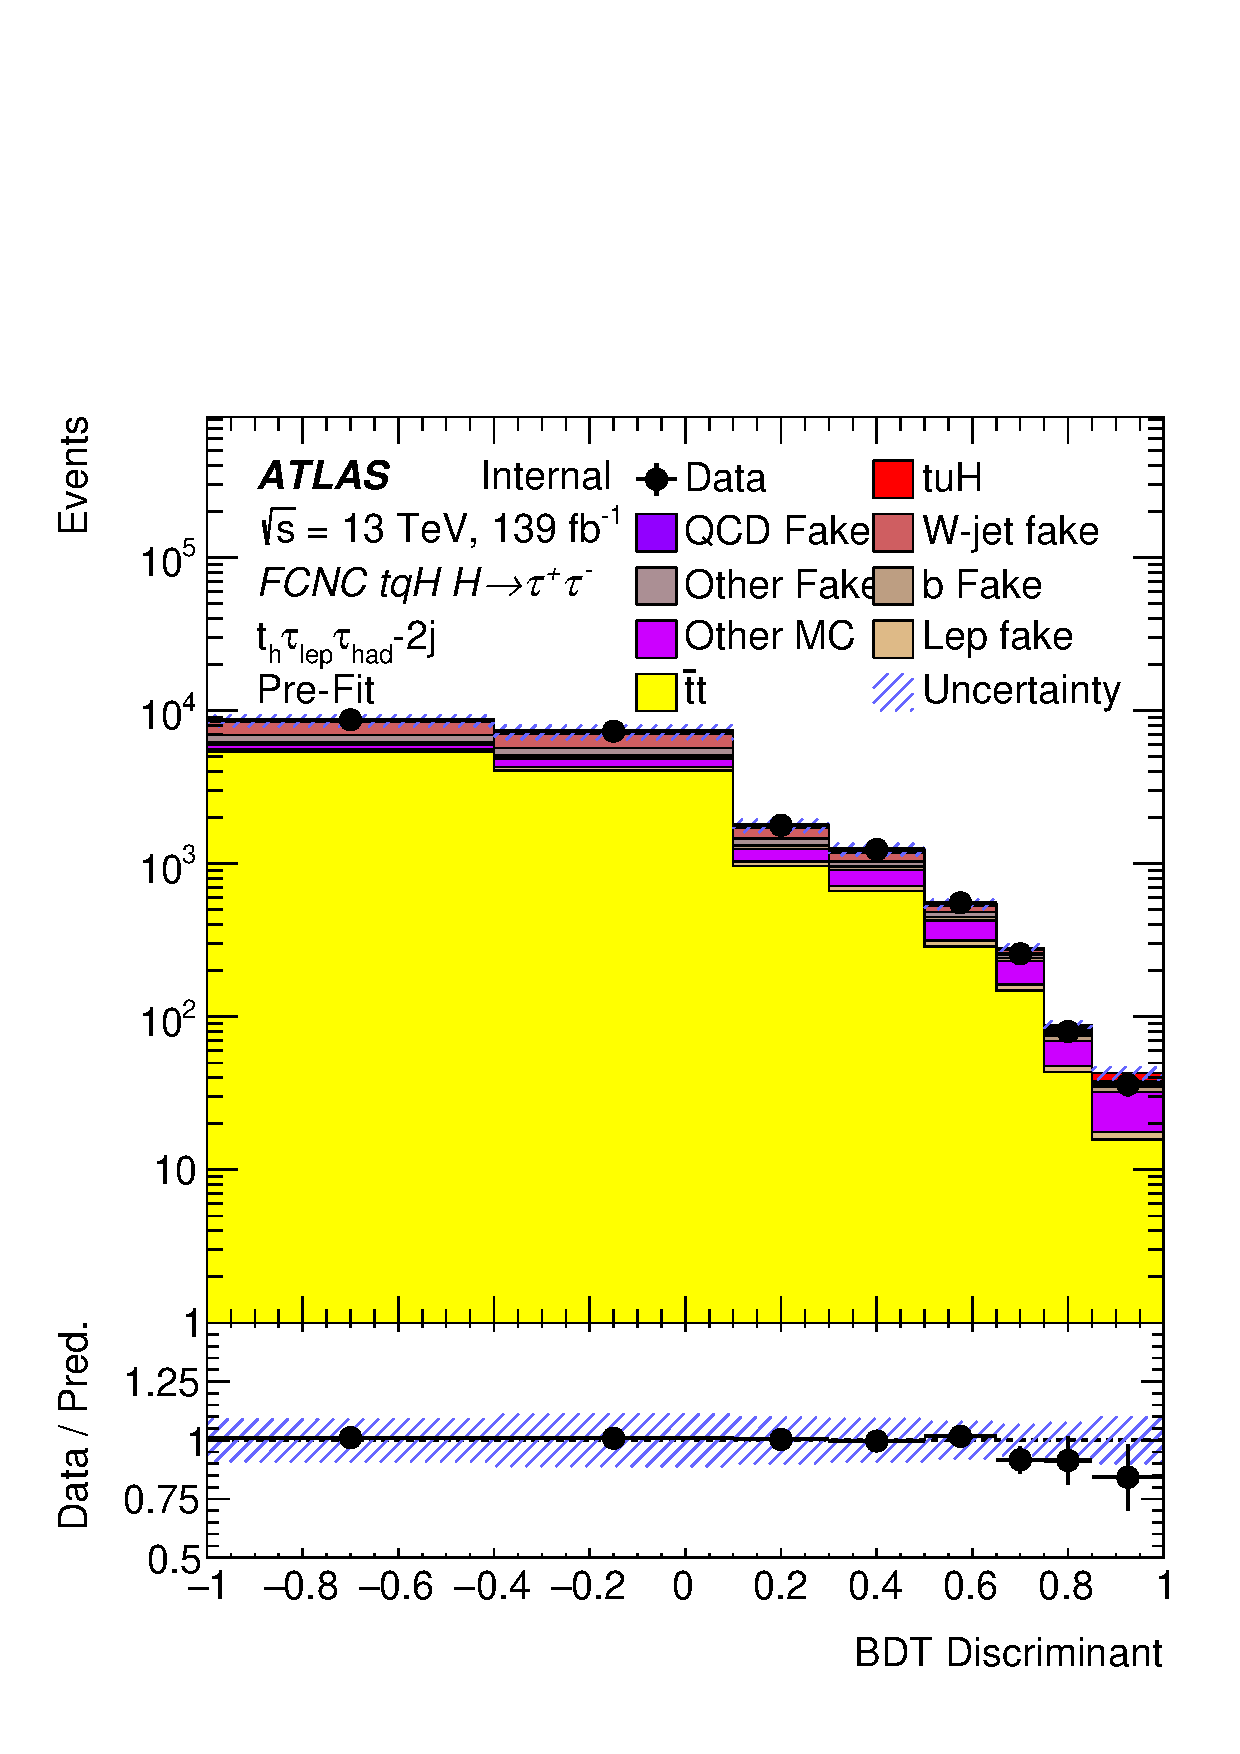
\includegraphics[width=0.25\textwidth]{figures/r21/thq1lntau/ROC/reg1l1tau1b2j_os.pdf}
\put(-70, 70){\textbf{(c3)}}\\
\includegraphics[page=4,width=0.25\textwidth]{figures/r21/thq1lntau/Wfake/doublecount/plots_NOMINAL/reg1l1tau1b3j_os/BDTG_test.pdf}
\put(-30, 80){\textbf{(d1)}}
\includegraphics[page=5,width=0.25\textwidth]{figures/r21/thq1lntau/Wfake/doublecount/plots_NOMINAL/reg1l1tau1b3j_os/BDTG_test.pdf}
\put(-30, 80){\textbf{(d2)}}
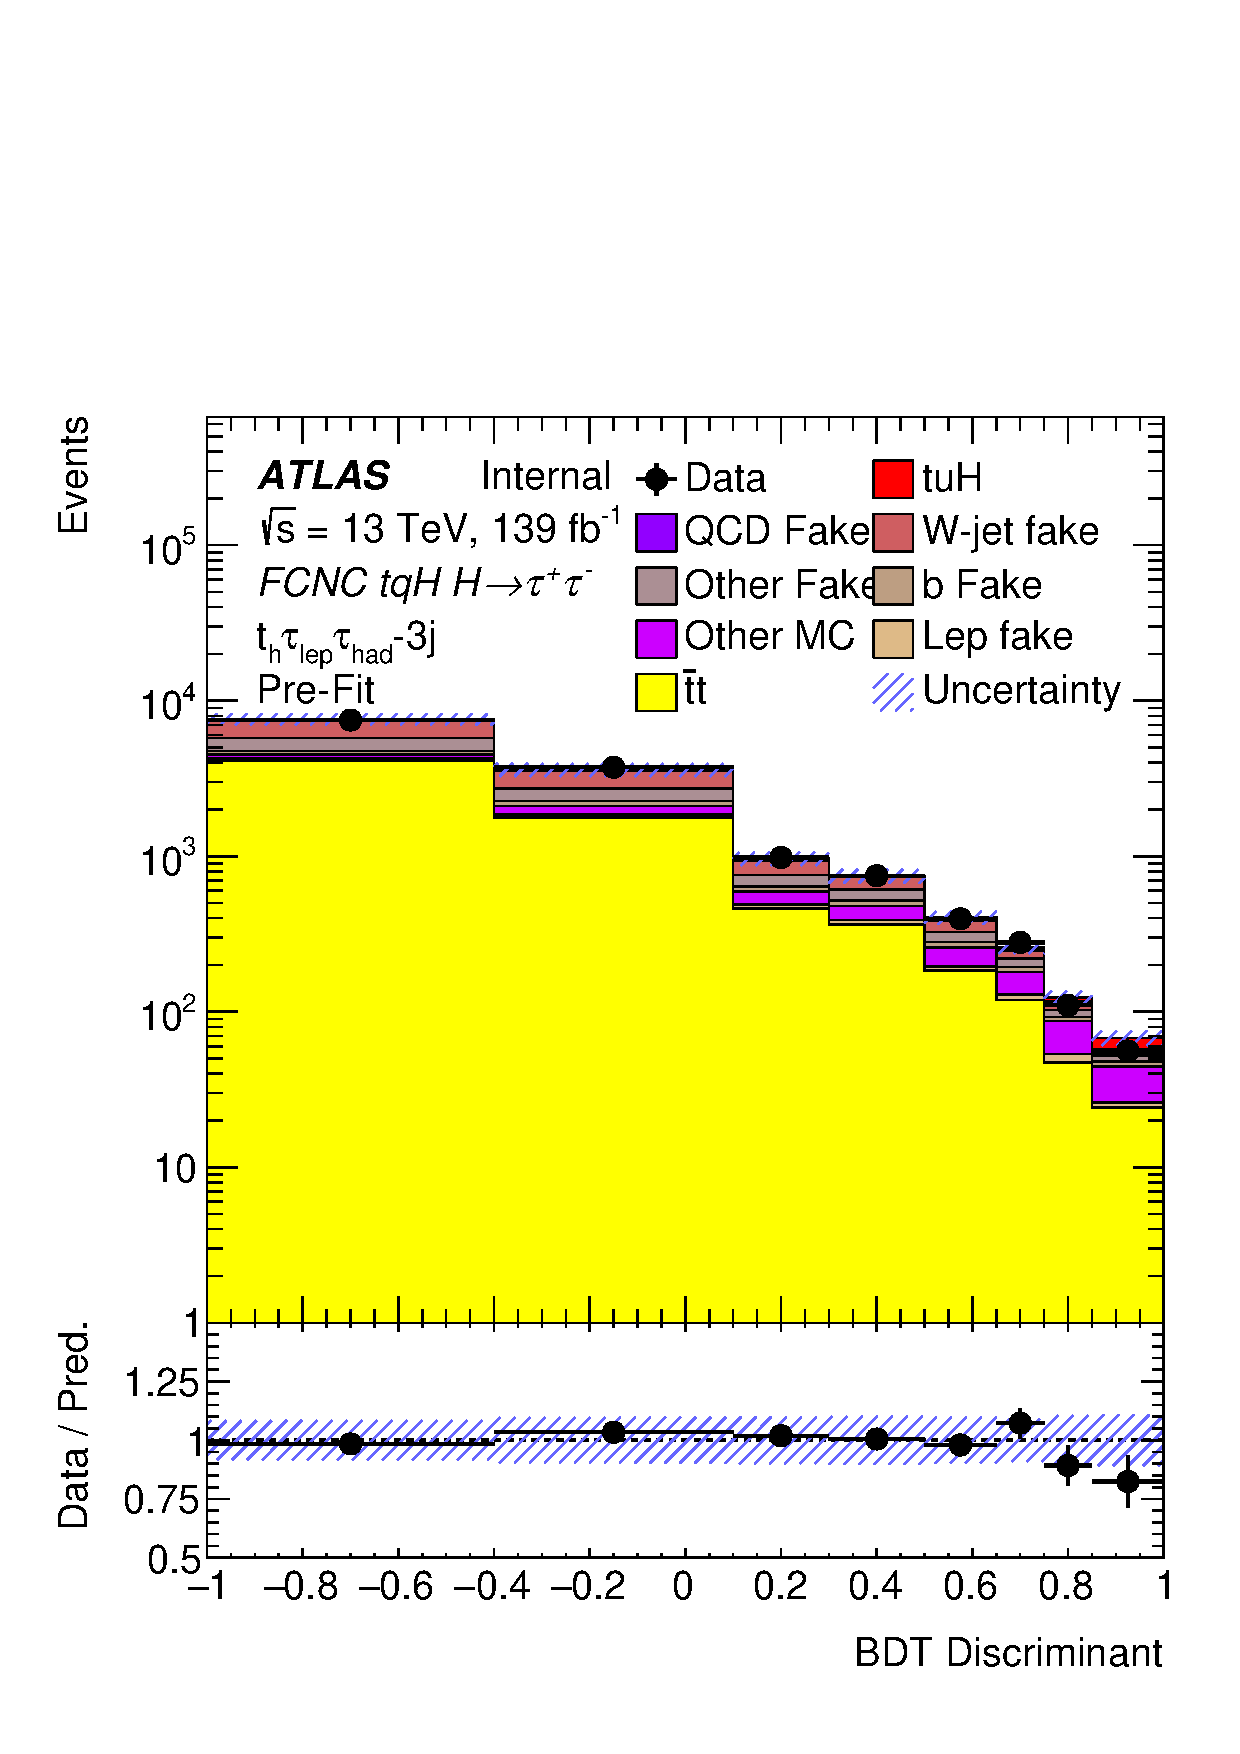
\includegraphics[width=0.25\textwidth]{figures/r21/thq1lntau/ROC/reg1l1tau1b3j_os.pdf}
\put(-70, 70){\textbf{(d3)}}\\
\includegraphics[page=4,width=0.25\textwidth]{figures/r21/thq1lntau/Wfake/doublecount/plots_NOMINAL/reg1l2tau1bnj_os/BDTG_test.pdf}
\put(-30, 80){\textbf{(e1)}}
\includegraphics[page=5,width=0.25\textwidth]{figures/r21/thq1lntau/Wfake/doublecount/plots_NOMINAL/reg1l2tau1bnj_os/BDTG_test.pdf}
\put(-30, 80){\textbf{(e2)}}
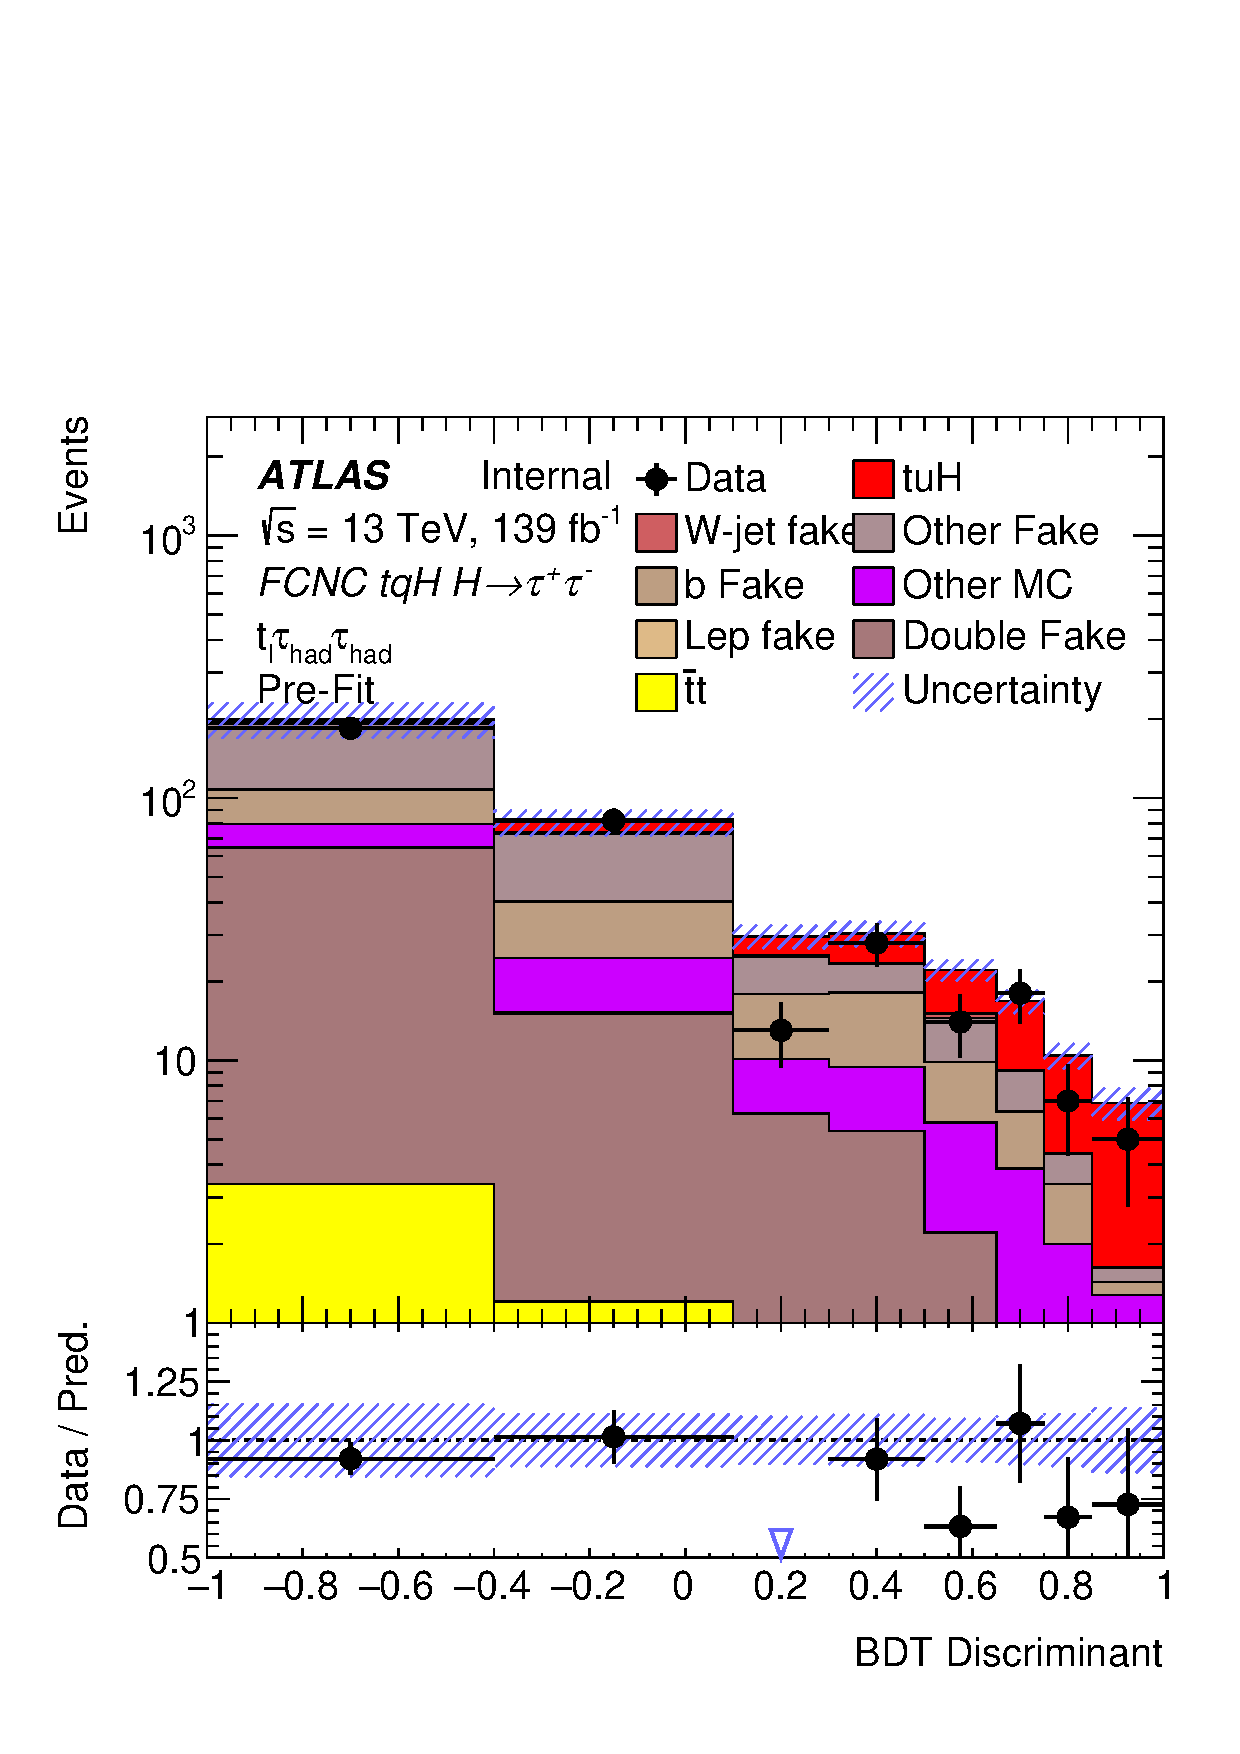
\includegraphics[width=0.25\textwidth]{figures/r21/thq1lntau/ROC/reg1l2tau1bnj_os.pdf}
\put(-70, 70){\textbf{(e3)}}\\
\caption{ The BDT output distributions for the background and TT signal (a1, b1, c1, d1, e1), background and ST signal (a2, b2, c2, d2, e2) and ROC curves (a3, b3, c3, d3, e3) in the STH $\thadhad$ (a1-3), TTH $\thadhad$ (b1-3), STH $\tlhad$ (c1-3), TTH $\tlhad$ (d1-3),  $l\thadhad$ (e1-3) channels. }% The Kolmogorov Test values for the training and testing BDT distributions are also indicated.
\label{fig:overtrain}
\end{figure}

The final yield and stat. only significance is shown in Table \ref{tab:yield} and Table \ref{tab:significance}


\input{tables/hadhad_significance_chart}
\centering
\begin{tabular}{|c|c|c|c|c|} \hline
 & 1l1tau1b1j ss e  highmet & 1l1tau1b1j ss e  lowmet & 1l1tau1b1j ss mu  highmet & 1l1tau1b1j ss mu  lowmet\\\hline
$\bar{t}t\to bWcH$ & $0.61$ & $0.23$ & $1.11$ & $0.34$\\\hline
$cg\to tH$ & $0.02$ & $0.01$ & $0.04$ & $0.01$\\\hline
tcH~merged~signal & $0.63$ & $0.24$ & $1.15$ & $0.35$\\\hline
$\bar{t}t\to bWuH$ & $0.64$ & $0.22$ & $1.18$ & $0.39$\\\hline
$ug\to tH$ & $0.05$ & $0.02$ & $0.28$ & $0.09$\\\hline
tuH~merged~signal & $0.70$ & $0.24$ & $1.45$ & $0.48$\\\hline
\end{tabular}
\begin{tabular}{|c|c|c|c|c|} \hline
 & 1l1tau1b2j os e  highmet & 1l1tau1b2j os e  lowmet & 1l1tau1b2j os mu  highmet & 1l1tau1b2j os mu  lowmet\\\hline
$\bar{t}t\to bWcH$ & $0.35$ & $0.13$ & $0.57$ & $0.25$\\\hline
$cg\to tH$ & $0.04$ & $0.01$ & $0.05$ & $0.01$\\\hline
tcH~merged~signal & $0.38$ & $0.14$ & $0.62$ & $0.27$\\\hline
$\bar{t}t\to bWuH$ & $0.36$ & $0.15$ & $0.60$ & $0.23$\\\hline
$ug\to tH$ & $0.21$ & $0.04$ & $0.35$ & $0.07$\\\hline
tuH~merged~signal & $0.55$ & $0.19$ & $0.92$ & $0.30$\\\hline
\end{tabular}
\begin{tabular}{|c|c|c|c|c|} \hline
 & 1l1tau1b2j ss e  highmet & 1l1tau1b2j ss e  lowmet & 1l1tau1b2j ss mu  highmet & 1l1tau1b2j ss mu  lowmet\\\hline
$\bar{t}t\to bWcH$ & $0.59$ & $0.19$ & $1.07$ & $0.35$\\\hline
$cg\to tH$ & $0.02$ & $0.00$ & $0.03$ & $0.01$\\\hline
tcH~merged~signal & $0.61$ & $0.20$ & $1.10$ & $0.36$\\\hline
$\bar{t}t\to bWuH$ & $0.64$ & $0.23$ & $1.13$ & $0.43$\\\hline
$ug\to tH$ & $0.03$ & $0.01$ & $0.23$ & $0.08$\\\hline
tuH~merged~signal & $0.68$ & $0.24$ & $1.35$ & $0.51$\\\hline
\end{tabular}
\begin{tabular}{|c|c|c|c|c|} \hline
 & 1l1tau1b3j os e  highmet & 1l1tau1b3j os e  lowmet & 1l1tau1b3j os mu  highmet & 1l1tau1b3j os mu  lowmet\\\hline
$\bar{t}t\to bWcH$ & $0.76$ & $0.28$ & $1.18$ & $0.50$\\\hline
$cg\to tH$ & $0.04$ & $0.01$ & $0.05$ & $0.02$\\\hline
tcH~merged~signal & $0.79$ & $0.29$ & $1.23$ & $0.51$\\\hline
$\bar{t}t\to bWuH$ & $0.77$ & $0.34$ & $1.28$ & $0.51$\\\hline
$ug\to tH$ & $0.22$ & $0.04$ & $0.30$ & $0.08$\\\hline
tuH~merged~signal & $0.98$ & $0.38$ & $1.58$ & $0.59$\\\hline
\end{tabular}
\begin{tabular}{|c|c|c|c|c|} \hline
 & 1l1tau1b3j ss e  highmet & 1l1tau1b3j ss e  lowmet & 1l1tau1b3j ss mu  highmet & 1l1tau1b3j ss mu  lowmet\\\hline
$\bar{t}t\to bWcH$ & $0.29$ & $0.09$ & $0.48$ & $0.16$\\\hline
$cg\to tH$ & $0.01$ & $0.00$ & $0.01$ & $0.00$\\\hline
tcH~merged~signal & $0.30$ & $0.09$ & $0.49$ & $0.17$\\\hline
$\bar{t}t\to bWuH$ & $0.31$ & $0.10$ & $0.54$ & $0.18$\\\hline
$ug\to tH$ & $0.03$ & $0.01$ & $0.06$ & $0.02$\\\hline
tuH~merged~signal & $0.33$ & $0.11$ & $0.60$ & $0.20$\\\hline
\end{tabular}
\begin{tabular}{|c|c|c|c|c|} \hline
 & 1l1tau2b1j ss e  highmet & 1l1tau2b1j ss e  lowmet & 1l1tau2b1j ss mu  highmet & 1l1tau2b1j ss mu  lowmet\\\hline
$\bar{t}t\to bWcH$ & $0.12$ & $0.07$ & $0.20$ & $0.06$\\\hline
$cg\to tH$ & $0.00$ & $0.00$ & $0.00$ & $0.00$\\\hline
tcH~merged~signal & $0.12$ & $0.07$ & $0.21$ & $0.06$\\\hline
$\bar{t}t\to bWuH$ & $0.04$ & $0.01$ & $0.08$ & $0.02$\\\hline
$ug\to tH$ & $0.01$ & $0.00$ & $0.02$ & $0.01$\\\hline
tuH~merged~signal & $0.04$ & $0.01$ & $0.10$ & $0.03$\\\hline
\end{tabular}
\begin{tabular}{|c|c|c|c|c|} \hline
 & 1l1tau2b2j os e  highmet & 1l1tau2b2j os e  lowmet & 1l1tau2b2j os mu  highmet & 1l1tau2b2j os mu  lowmet\\\hline
$\bar{t}t\to bWcH$ & $0.10$ & $0.03$ & $0.14$ & $0.07$\\\hline
$cg\to tH$ & $0.00$ & $0.00$ & $0.01$ & $0.00$\\\hline
tcH~merged~signal & $0.10$ & $0.03$ & $0.15$ & $0.07$\\\hline
$\bar{t}t\to bWuH$ & $0.03$ & $0.02$ & $0.07$ & $0.02$\\\hline
$ug\to tH$ & $0.02$ & $0.02$ & $0.03$ & $0.01$\\\hline
tuH~merged~signal & $0.04$ & $0.03$ & $0.10$ & $0.03$\\\hline
\end{tabular}
\begin{tabular}{|c|c|c|c|c|} \hline
 & 1l1tau2b2j ss e  highmet & 1l1tau2b2j ss e  lowmet & 1l1tau2b2j ss mu  highmet & 1l1tau2b2j ss mu  lowmet\\\hline
$\bar{t}t\to bWcH$ & $0.07$ & $0.06$ & $0.14$ & $0.04$\\\hline
$cg\to tH$ & $0.00$ & $0.00$ & $0.00$ & $0.00$\\\hline
tcH~merged~signal & $0.07$ & $0.06$ & $0.14$ & $0.04$\\\hline
$\bar{t}t\to bWuH$ & $0.04$ & $0.01$ & $0.07$ & $0.02$\\\hline
$ug\to tH$ & $0.00$ & $0.00$ & $0.02$ & $0.01$\\\hline
tuH~merged~signal & $0.05$ & $0.01$ & $0.08$ & $0.03$\\\hline
\end{tabular}
\begin{tabular}{|c|c|c|c|c|} \hline
 & 1l1tau2b3j os e  highmet & 1l1tau2b3j os e  lowmet & 1l1tau2b3j os mu  highmet & 1l1tau2b3j os mu  lowmet\\\hline
$\bar{t}t\to bWcH$ & $0.14$ & $0.03$ & $0.20$ & $0.10$\\\hline
$cg\to tH$ & $0.00$ & $0.00$ & $0.00$ & $0.00$\\\hline
tcH~merged~signal & $0.14$ & $0.03$ & $0.21$ & $0.10$\\\hline
$\bar{t}t\to bWuH$ & $0.07$ & $0.03$ & $0.10$ & $0.04$\\\hline
$ug\to tH$ & $0.01$ & $0.00$ & $0.03$ & $0.01$\\\hline
tuH~merged~signal & $0.08$ & $0.03$ & $0.13$ & $0.04$\\\hline
\end{tabular}
\begin{tabular}{|c|c|c|c|c|} \hline
 & 1l1tau2b3j ss e  highmet & 1l1tau2b3j ss e  lowmet & 1l1tau2b3j ss mu  highmet & 1l1tau2b3j ss mu  lowmet\\\hline
$\bar{t}t\to bWcH$ & $0.04$ & $0.01$ & $0.08$ & $0.02$\\\hline
$cg\to tH$ & $0.00$ & $0.00$ & $0.00$ & $0.00$\\\hline
tcH~merged~signal & $0.04$ & $0.01$ & $0.08$ & $0.02$\\\hline
$\bar{t}t\to bWuH$ & $0.03$ &  / & $0.04$ & $0.02$\\\hline
$ug\to tH$ & $0.00$ &  / & $0.01$ & $0.00$\\\hline
tuH~merged~signal & $0.03$ &  / & $0.04$ & $0.02$\\\hline
\end{tabular}
\begin{tabular}{|c|c|c|c|c|} \hline
 & 1l2tau1bnj os e  highmet & 1l2tau1bnj os e  lowmet & 1l2tau1bnj os mu  highmet & 1l2tau1bnj os mu  lowmet\\\hline
$\bar{t}t\to bWcH$ & $3.27$ & $1.47$ & $4.80$ & $2.71$\\\hline
$cg\to tH$ & $0.37$ & $0.12$ & $0.47$ & $0.26$\\\hline
tcH~merged~signal & $3.47$ & $1.55$ & $5.13$ & $2.88$\\\hline
$\bar{t}t\to bWuH$ & $3.55$ & $1.67$ & $5.04$ & $2.89$\\\hline
$ug\to tH$ & $0.65$ & $0.27$ & $2.30$ & $1.28$\\\hline
tuH~merged~signal & $3.92$ & $1.86$ & $6.76$ & $3.80$\\\hline
\end{tabular}
\begin{tabular}{|c|c|c|c|c|} \hline
 & 1l2tau1bnj ss e  highmet & 1l2tau1bnj ss e  lowmet & 1l2tau1bnj ss mu  highmet & 1l2tau1bnj ss mu  lowmet\\\hline
$\bar{t}t\to bWcH$ & $0.13$ & $0.15$ & $0.22$ & $0.14$\\\hline
$cg\to tH$ & $0.01$ & $0.01$ & $0.01$ & $0.01$\\\hline
tcH~merged~signal & $0.14$ & $0.16$ & $0.23$ & $0.14$\\\hline
$\bar{t}t\to bWuH$ & $0.18$ & $0.15$ & $0.24$ & $0.18$\\\hline
$ug\to tH$ & $0.05$ & $0.05$ & $0.07$ & $0.04$\\\hline
tuH~merged~signal & $0.22$ & $0.18$ & $0.31$ & $0.21$\\\hline
\end{tabular}
\begin{tabular}{|c|c|c|c|c|} \hline
 & 1l2tau2bnj os e  highmet & 1l2tau2bnj os e  lowmet & 1l2tau2bnj os mu  highmet & 1l2tau2bnj os mu  lowmet\\\hline
$\bar{t}t\to bWcH$ & $0.50$ & $0.60$ & $0.73$ & $0.38$\\\hline
$cg\to tH$ & $0.01$ & $0.02$ & $0.02$ & $0.01$\\\hline
tcH~merged~signal & $0.51$ & $0.61$ & $0.75$ & $0.39$\\\hline
$\bar{t}t\to bWuH$ & $0.15$ & $0.04$ & $0.18$ & $0.10$\\\hline
$ug\to tH$ & $0.01$ & $0.01$ & $0.07$ & $0.02$\\\hline
tuH~merged~signal & $0.16$ & $0.04$ & $0.25$ & $0.12$\\\hline
\end{tabular}
\begin{tabular}{|c|c|c|c|c|} \hline
 & 1l2tau2bnj ss e  highmet & 1l2tau2bnj ss mu  highmet & 1l2tau2bnj ss mu  lowmet & 1l1tau1b1j ss  highmet\\\hline
$\bar{t}t\to bWcH$ & $0.02$ & $0.03$ &  / & $1.26$\\\hline
$cg\to tH$ & $0.00$ & $0.01$ & $0.00$ & $0.05$\\\hline
tcH~merged~signal & $0.02$ & $0.03$ & $0.00$ & $1.31$\\\hline
$\bar{t}t\to bWuH$ & $0.01$ & $0.01$ &  / & $1.34$\\\hline
$ug\to tH$ &  / & $0.00$ &  / & $0.27$\\\hline
tuH~merged~signal & $0.01$ & $0.01$ &  / & $1.60$\\\hline
\end{tabular}
\begin{tabular}{|c|c|c|c|c|} \hline
 & 1l1tau1b1j ss  lowmet & 1l1tau1b2j os  highmet & 1l1tau1b2j os  lowmet & 1l1tau1b2j ss  highmet\\\hline
$\bar{t}t\to bWcH$ & $0.41$ & $0.67$ & $0.28$ & $1.22$\\\hline
$cg\to tH$ & $0.02$ & $0.06$ & $0.02$ & $0.03$\\\hline
tcH~merged~signal & $0.42$ & $0.73$ & $0.30$ & $1.26$\\\hline
$\bar{t}t\to bWuH$ & $0.45$ & $0.70$ & $0.28$ & $1.30$\\\hline
$ug\to tH$ & $0.09$ & $0.40$ & $0.08$ & $0.21$\\\hline
tuH~merged~signal & $0.53$ & $1.07$ & $0.35$ & $1.50$\\\hline
\end{tabular}
\begin{tabular}{|c|c|c|c|c|} \hline
 & 1l1tau1b2j ss  lowmet & 1l1tau1b3j os  highmet & 1l1tau1b3j os  lowmet & 1l1tau1b3j ss  highmet\\\hline
$\bar{t}t\to bWcH$ & $0.39$ & $1.40$ & $0.57$ & $0.56$\\\hline
$cg\to tH$ & $0.01$ & $0.06$ & $0.02$ & $0.01$\\\hline
tcH~merged~signal & $0.40$ & $1.46$ & $0.59$ & $0.57$\\\hline
$\bar{t}t\to bWuH$ & $0.48$ & $1.50$ & $0.61$ & $0.62$\\\hline
$ug\to tH$ & $0.07$ & $0.37$ & $0.09$ & $0.06$\\\hline
tuH~merged~signal & $0.55$ & $1.85$ & $0.70$ & $0.68$\\\hline
\end{tabular}
\begin{tabular}{|c|c|c|c|c|} \hline
 & 1l1tau1b3j ss  lowmet & 1l1tau2b1j ss  highmet & 1l1tau2b1j ss  lowmet & 1l1tau2b2j os  highmet\\\hline
$\bar{t}t\to bWcH$ & $0.19$ & $0.23$ & $0.08$ & $0.17$\\\hline
$cg\to tH$ & $0.00$ & $0.00$ & $0.00$ & $0.01$\\\hline
tcH~merged~signal & $0.19$ & $0.24$ & $0.08$ & $0.18$\\\hline
$\bar{t}t\to bWuH$ & $0.21$ & $0.09$ & $0.02$ & $0.07$\\\hline
$ug\to tH$ & $0.02$ & $0.02$ & $0.01$ & $0.04$\\\hline
tuH~merged~signal & $0.22$ & $0.11$ & $0.03$ & $0.11$\\\hline
\end{tabular}
\begin{tabular}{|c|c|c|c|c|} \hline
 & 1l1tau2b2j os  lowmet & 1l1tau2b2j ss  highmet & 1l1tau2b2j ss  lowmet & 1l1tau2b3j os  highmet\\\hline
$\bar{t}t\to bWcH$ & $0.07$ & $0.16$ & $0.06$ & $0.25$\\\hline
$cg\to tH$ & $0.00$ & $0.00$ & $0.00$ & $0.00$\\\hline
tcH~merged~signal & $0.07$ & $0.16$ & $0.06$ & $0.25$\\\hline
$\bar{t}t\to bWuH$ & $0.03$ & $0.08$ & $0.02$ & $0.13$\\\hline
$ug\to tH$ & $0.01$ & $0.02$ & $0.01$ & $0.03$\\\hline
tuH~merged~signal & $0.04$ & $0.09$ & $0.03$ & $0.15$\\\hline
\end{tabular}
\begin{tabular}{|c|c|c|c|c|} \hline
 & 1l1tau2b3j os  lowmet & 1l1tau2b3j ss  highmet & 1l1tau2b3j ss  lowmet & 1l2tau1bnj os  highmet\\\hline
$\bar{t}t\to bWcH$ & $0.10$ & $0.09$ & $0.02$ & $5.67$\\\hline
$cg\to tH$ & $0.00$ & $0.00$ & $0.00$ & $0.55$\\\hline
tcH~merged~signal & $0.10$ & $0.09$ & $0.02$ & $6.05$\\\hline
$\bar{t}t\to bWuH$ & $0.04$ & $0.05$ & $0.01$ & $6.01$\\\hline
$ug\to tH$ & $0.00$ & $0.01$ & $0.00$ & $2.33$\\\hline
tuH~merged~signal & $0.05$ & $0.05$ & $0.02$ & $7.71$\\\hline
\end{tabular}
\begin{tabular}{|c|c|c|c|c|} \hline
 & 1l2tau1bnj os  lowmet & 1l2tau1bnj ss  highmet & 1l2tau1bnj ss  lowmet & 1l2tau2bnj os  highmet\\\hline
$\bar{t}t\to bWcH$ & $3.00$ & $0.25$ & $0.19$ & $0.87$\\\hline
$cg\to tH$ & $0.27$ & $0.02$ & $0.01$ & $0.02$\\\hline
tcH~merged~signal & $3.19$ & $0.27$ & $0.19$ & $0.89$\\\hline
$\bar{t}t\to bWuH$ & $3.24$ & $0.29$ & $0.21$ & $0.22$\\\hline
$ug\to tH$ & $1.19$ & $0.09$ & $0.05$ & $0.06$\\\hline
tuH~merged~signal & $4.11$ & $0.37$ & $0.25$ & $0.29$\\\hline
\end{tabular}
\begin{tabular}{|c|c|c|c|c|} \hline
 & 1l2tau2bnj os  lowmet & 1l2tau2bnj ss  highmet & 1l2tau2bnj ss  lowmet & 1l1tau1b1j ss\\\hline
$\bar{t}t\to bWcH$ & $0.44$ & $0.03$ &  / & $1.33$\\\hline
$cg\to tH$ & $0.01$ & $0.00$ & $0.00$ & $0.05$\\\hline
tcH~merged~signal & $0.45$ & $0.03$ & $0.00$ & $1.37$\\\hline
$\bar{t}t\to bWuH$ & $0.10$ & $0.01$ &  / & $1.41$\\\hline
$ug\to tH$ & $0.02$ & $0.00$ &  / & $0.28$\\\hline
tuH~merged~signal & $0.12$ & $0.01$ &  / & $1.69$\\\hline
\end{tabular}
\begin{tabular}{|c|c|c|c|c|} \hline
 & 1l1tau1b2j os & 1l1tau1b2j ss & 1l1tau1b3j os & 1l1tau1b3j ss\\\hline
$\bar{t}t\to bWcH$ & $0.72$ & $1.28$ & $1.50$ & $0.59$\\\hline
$cg\to tH$ & $0.07$ & $0.04$ & $0.07$ & $0.01$\\\hline
tcH~merged~signal & $0.78$ & $1.32$ & $1.57$ & $0.60$\\\hline
$\bar{t}t\to bWuH$ & $0.74$ & $1.38$ & $1.61$ & $0.65$\\\hline
$ug\to tH$ & $0.40$ & $0.22$ & $0.38$ & $0.06$\\\hline
tuH~merged~signal & $1.11$ & $1.59$ & $1.98$ & $0.71$\\\hline
\end{tabular}
\begin{tabular}{|c|c|c|c|} \hline
 & 1l1tau2b1j ss & 1l1tau2b2j os & 1l1tau2b2j ss\\\hline
$\bar{t}t\to bWcH$ & $0.25$ & $0.18$ & $0.17$\\\hline
$cg\to tH$ & $0.00$ & $0.01$ & $0.00$\\\hline
tcH~merged~signal & $0.25$ & $0.19$ & $0.17$\\\hline
$\bar{t}t\to bWuH$ & $0.09$ & $0.08$ & $0.08$\\\hline
$ug\to tH$ & $0.02$ & $0.04$ & $0.02$\\\hline
tuH~merged~signal & $0.11$ & $0.11$ & $0.10$\\\hline
\end{tabular}
\begin{tabular}{|c|c|c|c|} \hline
 & 1l1tau2b3j os & 1l1tau2b3j ss & 1l2tau1bnj os\\\hline
$\bar{t}t\to bWcH$ & $0.26$ & $0.09$ & $6.34$\\\hline
$cg\to tH$ & $0.00$ & $0.00$ & $0.61$\\\hline
tcH~merged~signal & $0.27$ & $0.09$ & $6.77$\\\hline
$\bar{t}t\to bWuH$ & $0.13$ & $0.05$ & $6.74$\\\hline
$ug\to tH$ & $0.03$ & $0.01$ & $2.59$\\\hline
tuH~merged~signal & $0.16$ & $0.05$ & $8.64$\\\hline
\end{tabular}
\begin{tabular}{|c|c|c|c|} \hline
 & 1l2tau1bnj ss & 1l2tau2bnj os & 1l2tau2bnj ss\\\hline
$\bar{t}t\to bWcH$ & $0.30$ & $0.96$ & $0.03$\\\hline
$cg\to tH$ & $0.02$ & $0.02$ & $0.00$\\\hline
tcH~merged~signal & $0.31$ & $0.98$ & $0.03$\\\hline
$\bar{t}t\to bWuH$ & $0.35$ & $0.24$ & $0.01$\\\hline
$ug\to tH$ & $0.09$ & $0.06$ & $0.00$\\\hline
tuH~merged~signal & $0.43$ & $0.30$ & $0.01$\\\hline
\end{tabular}

\input{tables/hadhad_yield_chart}
\begin{table}
\footnotesize
\caption{The sample and data yield before the fit.}
\centering
\begin{tabular}{|c|c|c|c|c|} \hline
 & $l\thadhad$ ss & $l\thadhad$ os & STH $\tlhad$ ss & STH $\tlhad$ os\\\hline
data & $24.00\pm4.90$ & $28.00\pm5.29$ & $468.00\pm21.63$ & $6787.00\pm82.38$\\\hline
background & $28.34\pm1.91$ & $22.52\pm1.73$ & $459.96\pm8.96$ & $7004.75\pm32.28$\\\hline
$\bar{t}t\to bWcH$ & $0.29\pm0.04$ & $7.13\pm0.21$ & $7.05\pm0.20$ & $12.49\pm0.32$\\\hline
$cg\to tH$ & $0.01\pm0.00$ & $0.14\pm0.01$ & $0.15\pm0.01$ & $0.40\pm0.02$\\\hline
tcH~merged~signal & $0.30\pm0.04$ & $7.27\pm0.21$ & $7.20\pm0.20$ & $12.89\pm0.32$\\\hline
$\bar{t}t\to bWuH$ & $0.10\pm0.03$ & $0.84\pm0.07$ & $2.37\pm0.12$ & $3.92\pm0.17$\\\hline
$ug\to tH$ & $0.01\pm0.01$ & $0.23\pm0.03$ & $0.79\pm0.05$ & $1.79\pm0.09$\\\hline
tuH~merged~signal & $0.12\pm0.03$ & $1.07\pm0.08$ & $3.16\pm0.13$ & $5.72\pm0.20$\\\hline
\end{tabular}
\begin{tabular}{|c|c|c|c|c|} \hline
 & TTH $\tlhad$ ss & TTH $\tlhad$ os & $l\thadhad$ 2b ss & $l\thadhad$ 2b os\\\hline
data & $556.00\pm23.58$ & $4147.00\pm64.40$ & $75.00\pm8.66$ & $92.00\pm9.59$\\\hline
background & $511.26\pm9.76$ & $4342.91\pm24.01$ & $89.79\pm3.36$ & $79.48\pm3.09$\\\hline
$\bar{t}t\to bWcH$ & $4.61\pm0.17$ & $14.86\pm0.38$ & $0.22\pm0.04$ & $4.17\pm0.16$\\\hline
$cg\to tH$ & $0.06\pm0.01$ & $0.25\pm0.02$ & $0.00\pm0.00$ & $0.09\pm0.01$\\\hline
tcH~merged~signal & $4.68\pm0.17$ & $15.11\pm0.38$ & $0.23\pm0.04$ & $4.26\pm0.16$\\\hline
$\bar{t}t\to bWuH$ & $1.94\pm0.11$ & $3.97\pm0.18$ & $0.04\pm0.02$ & $0.44\pm0.05$\\\hline
$ug\to tH$ & $0.28\pm0.04$ & $1.11\pm0.08$ & $0.00\pm0.01$ & $0.23\pm0.03$\\\hline
tuH~merged~signal & $2.22\pm0.11$ & $5.08\pm0.20$ & $0.04\pm0.02$ & $0.67\pm0.06$\\\hline
\end{tabular}
\begin{tabular}{|c|c|c|c|c|} \hline
 & STH $\tlhad$ 2b ss & STH $\tlhad$ 2b os & TTH $\tlhad$ 2b ss & TTH $\tlhad$ 2b os\\\hline
data & $739.00\pm27.18$ & $9247.00\pm96.16$ & $622.00\pm24.94$ & $4689.00\pm68.48$\\\hline
background & $815.62\pm10.25$ & $9649.40\pm35.13$ & $575.99\pm8.45$ & $4865.38\pm24.75$\\\hline
$\bar{t}t\to bWcH$ & $1.88\pm0.10$ & $5.36\pm0.23$ & $1.21\pm0.08$ & $4.30\pm0.21$\\\hline
$cg\to tH$ & $0.02\pm0.00$ & $0.12\pm0.01$ & $0.02\pm0.00$ & $0.04\pm0.01$\\\hline
tcH~merged~signal & $1.90\pm0.10$ & $5.47\pm0.23$ & $1.23\pm0.08$ & $4.34\pm0.21$\\\hline
$\bar{t}t\to bWuH$ & $0.70\pm0.06$ & $1.28\pm0.10$ & $0.36\pm0.05$ & $1.09\pm0.10$\\\hline
$ug\to tH$ & $0.12\pm0.02$ & $0.50\pm0.05$ & $0.06\pm0.01$ & $0.27\pm0.04$\\\hline
tuH~merged~signal & $0.81\pm0.07$ & $1.78\pm0.11$ & $0.43\pm0.05$ & $1.36\pm0.10$\\\hline
\end{tabular}
\label{tab:yield}
\end{table}

